\documentclass[12pt,a4paper,oneside]{article}

\usepackage[utf8]{inputenc}
\usepackage[portuguese]{babel}
\usepackage[T1]{fontenc}
\usepackage{amsmath}
\usepackage{amsfonts}
\usepackage{amssymb}
\usepackage{graphicx}

\author{\\Universidade Federal de Goiás - UFG (Regional Jataí) \\Bacharelado em Ciência da Computação \\Inteligência Artificial \\Prof. Esdras Lins Bispo Jr.}

\title{
	{\sc \huge Lista de Exercícios 1} 
	\\{\tt Versão 3.0}
}

\begin{document}

\maketitle

\begin{enumerate}

	\item Leitura dos capítulos 1 e 2 (Russel e Norvig, 2013).
	
	\item {\bf [Russel 1.4]} Suponha que estendamos o programa ANALOGY de Evans para que possa alcançar 200 em um
teste de QI. Dessa forma teríamos um programa mais inteligente que um ser humano? Explique.	

	\item {\bf [Russel 1.7]} Até que ponto os sistemas seguintes são instâncias de inteligência artificial?
 		\begin{itemize}
 			\item Leitores de código de barra de supermercados.
			\item Menus de voz de telefones.
			\item Mecanismos de busca na Web.
			\item Algoritmos de roteamento da Internet que respondem dinamicamente ao estado da rede.
		\end{itemize}
	
	\item {\bf [Russel 1.11]} ``Sem dúvida, os computadores não podem ser inteligentes — eles só podem fazer o que seus programadores determinam.'' Esta última afirmação é verdadeira e implica a primeira?
	
	\item {\bf [Russel 1.12]} ``Sem dúvida, os animais não podem ser inteligentes — eles só podem fazer o que seus genes determinam.'' Esta última afirmação é verdadeira e implica a primeira?
	
	\item {\bf [Russel 1.13]} ``Sem dúvida, animais, seres humanos e computadores não podem ser inteligentes — eles só podem fazer o que seus átomos constituintes determinam, de acordo com as leis da física.'' Esta
última afirmação é verdadeira e implica a primeira?	

	\item Quatro pessoas precisam atravessar uma ponte que suporta no máximo duas pessoas ao mesmo tempo. É noite e eles não podem ver o caminho. Por sorte o grupo possui uma tocha que pode ser usada para iluminar o caminho enquanto eles atravessam a ponte. O tempo necessário para cada pessoa atravessar a ponte é respectivamente: 1, 2, 5 e 10 minutos. É possível que eles atravessem a ponte em 17 minutos?
	
		\begin{enumerate}
			\item Descreva o problema em termos de um problema de busca definindo o espaço de estados, o estado inicial, estado final, os operadores de transição entre os estados (ações) e o custo.
			\item Quantas vezes eles precisam atravessar a ponte?
			\item Construa um grafo do espaço de estados rotulando os arcos com os operadores de transição adequados.
		\end{enumerate}
	
	\item Em um labirinto, mostrado na figura a seguir, um robô é colocado na célula inicial indicada por ``E'' e deve encontrar um caminho até a saída, denotada pela letra ``S''. O robô não pode se mover na diagonal, somente acima, abaixo, direita e esquerda. Ele também não pode atravessar paredes (as linhas mais grossas da grade) ou as bordas do labirinto, de modo que ele é forçado a contornar obstáculos. Felizmente, o robô possui um mapa do ambiente. A solução é o caminho mais curto até a saída e todos os movimentos do robô possuem os mesmos custos.	
		
		\begin{center}
			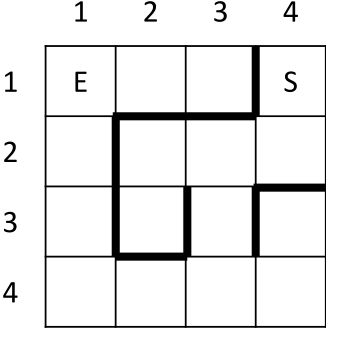
\includegraphics[width=5cm]{images/fig03.png}
		\end{center}		
		
		\begin{enumerate}
			\item Descreva o problema em termos de um problema de busca definindo o espaço de estados, o estado inicial, o estado final, os operadores de transição entre os estados (ações) e o custo.
			\item Construa um grafo do espaço de estados rotulando os arcos com os operadores de transição adequados.
		\end{enumerate}
		
\end{enumerate}

\section{Referências}

\begin{itemize}
	\item RUSSELL, S.; NORVIG, P. Inteligência Artificial. Rio de Janeiro: Editora Campus, 2013.
\end{itemize}

\end{document}